\documentclass[12pt, a4paper]{article}

\usepackage[utf8]{inputenc}
\usepackage{amsmath}
\usepackage{amsfonts}
\usepackage{amssymb}
\usepackage{graphicx}
\usepackage{hyperref}
\usepackage{setspace}
\usepackage{enumitem}
\usepackage{titlesec}
\usepackage{booktabs}
\usepackage{geometry}
\usepackage{tikz}
\usetikzlibrary{arrows.meta,positioning,shapes.geometric,fit,calc}

\geometry{
a4paper,
margin=1in
}

\title{
    \textbf{
        QUBO-Based Quantum and Quantum-Inspired Optimization\\
        for Real-Time NPC Squad Coordination
    }\\[0.4em]
    {\large A Comparative Study against Classical Baselines in the ShadowVale Game Testbed}
}

\author{
    \begin{tabular}{cc}
        Tran Tuan Anh & Nguyen Dang Khoa \\[0.3em]
        Nguyen Dinh Tai & Nguyen Cong Thinh \\[0.8em]
        \multicolumn{2}{c}{\textit{Supervisor: Lai Duc Hung}}
    \end{tabular}
}

\date{}
% ---------- Document formatting ----------

\setstretch{1.15}
\setlength{\parindent}{0pt}
\setlength{\parskip}{6pt}
\setlength{\emergencystretch}{2em}

\titleformat{\section}
{\large\bfseries}
{\thesection.}
{0.5em}
{}

\titleformat{\subsection}
{\normalsize\bfseries}
{\thesubsection}
{0.5em}
{}

\setlist[itemize]{
leftmargin=2em,
itemsep=2pt,
topsep=3pt
}

\begin{document}

\maketitle

% ============================================================
\section*{Scientific Abstract}

Real-time tactical coordination of multiple non-player characters (NPCs) in video games can be formulated as a combinatorial optimization problem when agents must simultaneously select tactical positions, cover escape routes, reduce spatial redundancy, and react to a moving player.

Traditional game AI techniques such as Finite State Machines (FSMs), Behavior Trees (BTs), influence maps, and greedy assignment algorithms are computationally efficient and widely applicable. However, when coordination decisions involve many interacting agents and tactical positions, purely local heuristics may produce suboptimal or predictable group behavior.

This research introduces \textit{ShadowVale}, a 2.5D tactical stealth-survival game used as an experimental testbed for studying optimization-based NPC coordination. Tactical assignment decisions are formulated as a Quadratic Unconstrained Binary Optimization (QUBO) problem and transformed, when required, into an equivalent Ising representation.

The study compares several optimization approaches: the Quantum Approximate Optimization Algorithm (QAOA) executed on a quantum simulator, Simulated Quantum Annealing (SQA), and a Quantum-Inspired Evolutionary Algorithm (QIEA). These methods are compared against classical baselines, namely Greedy Assignment, Greedy with local search, tabu search, a Genetic Algorithm (GA), and Simulated Annealing (SA) over bits and over assignments, and against PBIL, an ablation of QIEA without Q-bits; exhaustive enumeration, an exact set-reduction solver and branch and bound provide the optimum on small and game-size instances.

Evaluation is conducted using optimization metrics such as solution quality, feasibility rate, wall-clock latency, and scalability. In addition, in-game telemetry is used to evaluate whether changes in optimization quality produce observable differences in tactical coverage, player escape time, and NPC coordination.

In the official run (exp-v2: 3{,}447 assignment problems recorded inside the game, all with a proven optimum, 1{,}350 generated instances of up to 1{,}200 binary variables, and two public datasets, QAPLIB and Moving AI), the strongest method within the 120\,ms budget is classical: tabu search finds the optimum in 99.9\,\% of the runs on in-game problems, and a millisecond of local search after Greedy reduces Greedy's mean gap from 2.8\,\% to 0.27\,\%. Because only travel cost depends on the agent, the exact problem reduces to choosing a set of positions and solving a linear assignment, which proves every game-size optimum in about 0.1\,s. The quantum-inspired QIEA is as accurate as a genetic algorithm (0.11\,\% on in-game problems) and as PBIL, an ablation without Q-bits; SA and SQA, which flip raw bits of the one-hot QUBO, are less accurate than Greedy, whereas annealing over assignments is not. Read from the statevector, simulated QAOA does not produce the optimum more often than uniform sampling of valid assignments, with either the standard or a constraint-preserving mixer. In 1{,}800 paired replays of scripted exploits on the final build, the solver changed capture rates by up to 36 points against one exploit but in opposite directions across exploits, and coordinating at all mattered as much as the choice of solver.

The objective of this work is not to claim quantum computational advantage, but to determine whether QUBO-based modeling provides a practical and reproducible framework for multi-agent tactical decision making and to identify the problem-size regimes in which quantum, quantum-inspired, and classical optimization methods are computationally viable.

% ============================================================
\section*{Background and Problem Statement}

Multi-agent coordination is an important problem in Game Artificial Intelligence (Game AI). While controlling a single NPC may be achieved using state machines, behavior trees, utility systems, or navigation algorithms, coordinating a squad introduces additional dependencies between agents.

For example, when a player is detected, a squad may need to perform several actions simultaneously:

\begin{itemize}
\item occupy different cover positions,
\item block likely escape paths,
\item create flanking angles,
\item avoid assigning multiple agents to the same tactical location,
\item maintain line-of-sight or cross-support,
\item minimize unnecessary travel distance.
\end{itemize}

These decisions cannot always be optimized independently because the usefulness of one NPC's position may depend on the positions selected by other NPCs.

This interaction naturally creates quadratic relationships between assignment decisions and motivates the use of combinatorial optimization models.

The resulting tactical assignment problem is related to generalized assignment and quadratic assignment problems; the quadratic assignment problem is NP-hard \cite{Sahni1976}. With pairwise interactions and multiple constraints, the general optimization problem can become computationally difficult as the number of agents and candidate positions grows.

However, a game system also imposes practical latency constraints.

A game running at 60 FPS has approximately 16.7 milliseconds per rendered frame, while a game running at 30 FPS has approximately 33.3 milliseconds. Nevertheless, a high-level squad coordinator does not necessarily need to execute every frame.

In ShadowVale, low-level movement and combat remain inside the Unity game loop, while squad-level tactical optimization is executed asynchronously when important events occur, such as:

\begin{itemize}
\item the player being detected,
\item the current formation becoming invalid,
\item a tactical position becoming unavailable,
\item an NPC being eliminated,
\item a configurable coordination interval being reached.
\end{itemize}

Therefore, this research evaluates solver latency independently from frame rendering and investigates which algorithms are practical under different tactical decision budgets.

% ============================================================
\section*{Research Questions}

The study is structured around the following research questions:

\begin{enumerate}
\item \textbf{RQ1:} Can tactical NPC assignment in ShadowVale be represented effectively as a QUBO/Ising optimization problem?

\item \textbf{RQ2:} How do QAOA, SQA, and QIEA compare with classical baselines (Greedy Assignment, GA, and SA) in terms of solution quality and constraint satisfaction under equal computational budgets?

\item \textbf{RQ3:} How does problem size affect the latency and solution quality of each optimization method?

\item \textbf{RQ4:} What problem-size regimes are practically feasible for QAOA simulation compared with classical and quantum-inspired methods?

\item \textbf{RQ5:} Do improvements in mathematical coordination quality produce measurable differences in actual gameplay telemetry?

\end{enumerate}

The research focuses specifically on high-level tactical assignment. It does not attempt to replace Unity navigation, local obstacle avoidance, animation control, or individual NPC behavior logic.

% ============================================================
\section*{Main Research Question}

Can real-time tactical assignment of an NPC squad be formulated as a QUBO/Ising problem such that quantum (simulated), simulated-quantum, and quantum-inspired optimizers produce assignments of competitive quality to classical baselines, and within which problem-size regime does each method fit a practical coordination latency budget?

% ============================================================
\section*{Research Objectives}

\begin{itemize}
\item \textbf{O1} -- Formulate squad tactical assignment (cover occupation, escape-route blocking, flanking) as a QUBO with tunable weights and penalty terms. (RQ1)
\item \textbf{O2} -- Implement a common solver interface with classical baselines (Greedy, Greedy with local search, tabu search, GA, SA), SQA, QIEA, and QAOA on a simulator, plus exact reference solvers. (RQ2)
\item \textbf{O3} -- Build a seeded, reproducible benchmark of tactical instances with controlled size (agents $A$, nodes $N$) and chokepoint density, complemented by instances recorded in the game and two public datasets. (RQ3)
\item \textbf{O4} -- Measure solution quality, feasibility, latency, and scalability, and identify the viable problem-size regime of each solver. (RQ3, RQ4)
\item \textbf{O5} -- Integrate the best-performing solver into ShadowVale and evaluate its gameplay effects through telemetry and a pilot playtest. (RQ5)
\end{itemize}

% ============================================================
\section*{Scope}

The study considers single-player NPC squads of 2 to 12 agents. In play, a combat group of at most 8 agents is assigned over a local tactical subgraph of 24 nodes around the player, i.e.\ at most $n = 192$ binary variables; the benchmark extends to 12 agents over 100 nodes ($n = 1{,}200$). In-game coordination runs under a latency budget of 120\,ms. Standard QAOA is restricted to instances of at most $n = 18$ variables on our statevector simulator and is evaluated offline; a constraint-preserving variant is simulated on larger instances in its feasible subspace.

Out of scope are claims of quantum hardware speed-up, experiments on physical quantum hardware (a small QPU run is an optional feasibility demonstration only), low-level navigation and animation, and large-scale reinforcement learning.

% ============================================================
\section*{Literature Review and Precedent Systems}

\subsection*{Multi-Agent AI in Games}

Traditional Game AI frequently uses Finite State Machines and Behavior Trees because they are computationally efficient, explainable, and easy to integrate with real-time game engines.

Such systems work well for individual agents. However, explicit cooperation between multiple agents often requires additional mechanisms such as shared blackboards, influence maps, squad managers, utility functions, or centralized planners.

Commercial titles illustrate this layering. F.E.A.R. combined FSMs with goal-oriented action planning to produce emergent squad behavior \cite{Orkin2006}, and Killzone selected combat positions at runtime by evaluating annotated waypoints with tactical scoring functions \cite{Straatman2005}. Game AI textbooks describe influence maps, utility-based selection, and centralized squad managers as the standard tools for group decisions \cite{Yannakakis2018}. These systems usually choose positions per agent or greedily and do not optimize the pairwise interactions between assignments globally.

Multi-Agent Path Finding (MAPF) studies the related problem of finding collision-free routes for several agents operating in a shared environment. Conflict-Based Search (CBS), for example, uses a two-level search architecture to resolve conflicts while maintaining optimality \cite{Sharon2015}.

The optimization problem considered in ShadowVale is different from pure MAPF. Instead of solving complete collision-free trajectories, the proposed coordinator selects high-level tactical destinations. Unity's navigation layer subsequently handles path execution.

This separation reduces the optimization space while allowing tactical interactions between NPC assignments to be studied independently.

% ------------------------------------------------------------
\subsection*{QUBO and the Ising Model}

The Ising model describes binary spin variables

$$
s_i \in \{-1,+1\}
$$

with an energy function of the form

$$
H(s)
=
\sum_i h_i s_i
+
\sum_{i<j} J_{ij}s_i s_j.
$$

Here, $h_i$ represents an individual spin bias and $J_{ij}$ represents a pairwise interaction.

Many discrete optimization problems can be transformed into Ising or QUBO formulations \cite{Lucas2014}.

A QUBO problem uses binary variables

$$
x_i \in \{0,1\}
$$

and seeks to minimize an objective of the form

$$
E(x)
=
\sum_i q_i x_i
+
\sum_{i<j} q_{ij}x_i x_j.
$$

Equivalently, a QUBO may be written as

$$
E(x)=x^TQx,
$$

provided that the matrix convention for off-diagonal coefficients is defined consistently.

If $Q$ is symmetric, pairwise coefficients are divided between $Q_{ij}$ and $Q_{ji}$ so that quadratic terms are not counted twice.

Binary and Ising variables can be converted using

$$
s_i = 2x_i-1
$$

or equivalently

$$
x_i = \frac{s_i+1}{2}.
$$


Glover, Kochenberger, and Du give a tutorial treatment of QUBO modeling, including one-hot encodings of assignment constraints through quadratic penalties and QUBO formulations of the quadratic assignment problem \cite{Glover2019}. The formulation in this work follows this standard penalty construction; its contribution lies in the domain-specific tactical terms and in the analysis of the penalty weight, not in the encoding itself.

QUBO is particularly useful for the ShadowVale problem because tactical rewards can be represented by linear terms while interactions between agent assignments can be represented by quadratic terms.

% ------------------------------------------------------------
\subsection*{Quantum and Quantum-Inspired Optimization}

Quantum optimization methods attempt to use quantum-mechanical computational models for solving discrete optimization problems.

QAOA was introduced by Farhi, Goldstone, and Gutmann as a variational quantum algorithm for approximate combinatorial optimization \cite{Farhi2014}.

Quantum annealing approaches optimize Ising-like energy functions by evolving a system from an easier initial Hamiltonian toward a problem Hamiltonian \cite{Kadowaki1998}.

Because this project is designed to operate without requiring access to physical quantum hardware, quantum annealing behavior is studied through classical simulation methods.

Quantum-inspired algorithms differ from actual quantum algorithms. They execute entirely on classical hardware while borrowing concepts such as probabilistic Q-bit representations and rotation operators.

One example is the Quantum-Inspired Evolutionary Algorithm introduced by Han and Kim \cite{HanKim2002}.

Quantum annealing has already been applied to assignment-like problems outside games. In traffic-flow optimization, for example, each vehicle selects one route from a small candidate set while quadratic terms penalize congestion between vehicles \cite{Neukart2017}, a structure very close to the tactical assignment studied here. In games, quantum computation has so far been used mainly for procedural content generation rather than NPC decision making \cite{Wootton2020}.

Therefore, this project distinguishes three categories:

\begin{itemize}
\item \textbf{Quantum algorithm executed on a simulator:} QAOA,
\item \textbf{Classical simulation of quantum annealing dynamics:} SQA,
\item \textbf{Quantum-inspired classical optimization:} QIEA.
\end{itemize}

Classical Greedy Assignment, a Genetic Algorithm, and Simulated Annealing are retained as baselines.

% ------------------------------------------------------------
\subsection*{Research Gap}

Existing game AI coordinates squads with FSMs, behavior trees, utility functions, and greedy position selection \cite{Orkin2006,Straatman2005,Yannakakis2018}, while MAPF research optimizes collision-free trajectories rather than tactical destinations \cite{Sharon2015}. QUBO modeling of assignment problems is well established \cite{Lucas2014,Glover2019}, and quantum annealing has been applied to assignment-like problems outside games \cite{Neukart2017}, but quantum work in games has focused on content generation \cite{Wootton2020}. To our knowledge, little prior work formulates real-time NPC squad tactical assignment as a QUBO and compares quantum, simulated-quantum, quantum-inspired, and classical solvers on identical instances under a game latency budget. This work addresses that gap.

% ============================================================
\section*{Mathematical Formulation of Tactical Coordination}

\subsection*{Sets and Decision Variables}

Let

$$
I=\{1,2,\ldots,N\}
$$

be the set of NPC agents participating in the current tactical coordination event.

Let $R_i$ denote the set of candidate tactical positions available to agent $i$.

Instead of allowing every NPC to consider every navigable node in the map, ShadowVale performs candidate filtering before optimization.

Candidate positions may include:

\begin{itemize}
\item nearby cover points,
\item escape-route chokepoints,
\item flanking positions,
\item positions with useful line-of-sight,
\item defensive positions around an objective.
\end{itemize}

For every valid agent-position pair $(i,r)$, define

$$
x_{i,r}\in\{0,1\}.
$$

The variable is interpreted as

$$
x_{i,r}
=
\begin{cases}
1, & \text{if agent } i \text{ is assigned to position } r,\\
0, & \text{otherwise}.
\end{cases}
$$

The total number of binary variables is

$$
n=\sum_{i\in I}|R_i|.
$$

% ------------------------------------------------------------
\subsection*{Tactical Utility}

Each assignment has a tactical utility

$$
u_{i,r}.
$$

The value may combine several normalized features, for example:

$$
u_{i,r}
=
w_1 C_{r}
+
w_2 F_{i,r}
+
w_3 L_{i,r}
-
w_4 D_{i,r},
$$

where:

\begin{itemize}
\item $C_r$ is the value of covering a tactical region,
\item $F_{i,r}$ represents flanking quality,
\item $L_{i,r}$ represents line-of-sight quality,
\item $D_{i,r}$ represents travel cost,
\item $w_1,\ldots,w_4$ are configurable weights.
\end{itemize}

The total tactical reward is

$$
R_{\text{tac}}
=
\sum_{i\in I}
\sum_{r\in R_i}
u_{i,r}x_{i,r}.
$$

Because QUBO is formulated as minimization, tactical utility enters the final energy function with a negative sign.

% ------------------------------------------------------------
\subsection*{Spatial Redundancy and Conflict Penalty}

Two assignments may conflict or provide redundant tactical coverage.

Let

$$
c_{(i,r),(j,r')}
\geq 0
$$

represent the degree of conflict between assigning agent $i$ to $r$ and agent $j$ to $r'$.

Examples include:

\begin{itemize}
\item assigning two NPCs to the same cover point,
\item selecting positions that are too close together,
\item blocking the same narrow corridor redundantly,
\item producing almost identical firing angles.
\end{itemize}

The corresponding quadratic penalty is

$$
P_{\text{overlap}}
=
\lambda
\sum_{i<j}
\sum_{r\in R_i}
\sum_{r'\in R_j}
c_{(i,r),(j,r')}
x_{i,r}x_{j,r'},
$$

where $\lambda > 0$ controls the importance of reducing redundancy.

When two agents select the same position ($r = r'$), the conflict coefficient is set large enough that the term acts as an at-most-one-agent-per-position constraint rather than a soft preference. The remaining conflict types are soft penalties.

% ------------------------------------------------------------
\subsection*{One-Agent-One-Task Constraint}

Each participating NPC must receive exactly one tactical assignment:

$$
\sum_{r\in R_i}x_{i,r}=1,
\qquad
\forall i\in I.
$$

QUBO does not directly contain equality constraints, so the constraint is transformed into a quadratic penalty:

$$
P_{\text{assignment}}
=
M
\sum_{i\in I}
\left(
1-
\sum_{r\in R_i}x_{i,r}
\right)^2,
$$

where $M>0$ must dominate both the tactical rewards and the conflict terms. In the implementation (see ``Instantiation in ShadowVale'') let $L=\max_r(w_{\text{cov}}\mathrm{cov}_r+w_{\text{cover}}q_r)$ be the largest linear reward, $D=w_{\text{dist}}\max_{i,r}d_{i,r}$ the largest travel cost, $P^+=w_{\text{flank}}\max\mathrm{flk}$ the largest pairwise reward and $P^-=w_{\text{red}}\max\mathrm{ovl}$ the largest pairwise cost, and set
$$
M = 1 + L + 2(|I|-1)P^+ + D + (|I|-1)P^- .
$$
Any infeasible bit vector can be turned into a feasible one by steps that each lower the energy: (i) an agent holding $k\ge 2$ positions drops one, which removes at least $M$ of penalty and at most $L+2(|I|-1)P^+$ of reward (the flanking rewards it shared with other agents included); (ii) when two agents share a position, one of them moves to a free position, a two-bit move that removes $M$ of penalty and changes the objective by at most $L+(|I|-1)P^+ + D+(|I|-1)P^-$; (iii) an agent without a position takes a free one, losing at most $D+(|I|-1)P^-$. Hence every infeasible vector has a higher energy than some feasible one, and every global minimum is feasible. This is weaker than the claim of the first version that every single-bit-flip local minimum is feasible: step (ii) needs two flips, and with flanking rewards (negative energy coefficients) a one-bit argument does not hold. The bound is verified exhaustively by unit tests on small generated instances.

Expanding the penalty for one agent gives

$$
\left(
1-\sum_r x_{i,r}
\right)^2
=
1
-
2\sum_r x_{i,r}
+
\left(\sum_r x_{i,r}\right)^2.
$$

Because

$$
x_{i,r}^2=x_{i,r}
$$

for binary variables,

$$
\left(
1-\sum_r x_{i,r}
\right)^2
=
1
-
\sum_r x_{i,r}
+
2\sum_{r<r'}x_{i,r}x_{i,r'}.
$$

The constant term does not affect the optimizer and can therefore be removed when constructing the QUBO matrix.

% ------------------------------------------------------------
\subsection*{Complete QUBO Objective}

Combining tactical reward, redundancy penalty, and assignment constraints produces

$$
E(x)
=
-
R_{\text{tac}}
+
P_{\text{overlap}}
+
P_{\text{assignment}}.
$$

Therefore,

$$
\boxed{
E(x)
=
-
\sum_i\sum_{r\in R_i}
u_{i,r}x_{i,r}
+
\lambda
\sum_{i<j}
\sum_{r\in R_i}
\sum_{r'\in R_j}
c_{(i,r),(j,r')}
x_{i,r}x_{j,r'}
+
M
\sum_i
\left(
1-\sum_{r\in R_i}x_{i,r}
\right)^2
}
$$

This objective can be converted into a standard QUBO matrix $Q$ and supplied to each compatible optimizer.

The exact values of $\lambda$ and $M$ are treated as experimental parameters and are calibrated to prevent constraint violations without allowing penalties to dominate all meaningful tactical differences.

% ------------------------------------------------------------
\subsection*{Instantiation in ShadowVale}

In the implementation every agent of a combat group may take any node of a local subgraph $V$ of the tactical navigation graph of at most 24 nodes: every agent's current node, filled up with the nodes nearest to the player's last known position ($19 \le |V| \le 24$ in play). Hence $R_i = V$ for all agents and $n = A\,|V|$. Escape nodes $X \subseteq V$ are the boundary ring of the subgraph together with any map chokepoint inside it. With $\mathrm{vis}(r, e)$ the line of sight between nodes (ray-cast once per map load), the objective $F$ maximised by the coordinator is
$$
\begin{aligned}
F(x) ={}& w_{\text{cov}}\sum_{i,r} \mathrm{cov}_r x_{i,r}
+ w_{\text{cover}}\sum_{i,r} q_r x_{i,r}
- w_{\text{dist}}\sum_{i,r} d_{i,r} x_{i,r}\\
&- w_{\text{red}}\sum_{i<j}\sum_{r\neq r'} \mathrm{ovl}_{r,r'} x_{i,r}x_{j,r'}
+ w_{\text{flank}}\sum_{i<j}\sum_{r\neq r'} \mathrm{flk}_{r,r'} x_{i,r}x_{j,r'},
\end{aligned}
$$
where $\mathrm{cov}_r$ is the number of escape nodes visible from $r$, $\mathrm{ovl}_{r,r'}$ the number visible from both positions (redundancy), $\mathrm{flk}_{r,r'} \in [0,1]$ equals 1 when the two positions lie on opposite sides of the player (flanking), $q_r = \mathrm{is\_cover}_r \cdot \max(0, \cos\angle(\text{facing}_r, r \to \text{player}))$ is the cover quality, and $d_{i,r}$ is the travel cost of agent $i$ to $r$ in graph hops. The weights are $(w_{\text{cov}}, w_{\text{red}}, w_{\text{flank}}, w_{\text{cover}}, w_{\text{dist}}) = (1, 0.5, 1, 0.5, 0.1)$, read from the content bundle. The energy is $E(x) = -F(x) + M\sum_i(1-\sum_r x_{i,r})^2 + M\sum_r\sum_{i<j} x_{i,r}x_{j,r}$, with $M$ computed per instance from the bound above. Unit tests verify on every generated instance that $E + \text{offset} = -F$ on feasible assignments and that every infeasible assignment has a higher energy than the best feasible one. The QUBO is built in C\# inside Unity and, for the benchmark, in Python; a parity test requires both to agree to $10^{-9}$.

\textbf{Node-only structure.} Only the travel cost $d_{i,r}$ depends on the agent; coverage, cover quality, redundancy and flanking depend on the positions alone. Writing $S$ for the set of positions taken,
$$
\max_x F = \max_{|S|=|I|}\Big[G(S) - w_{\text{dist}}\min_{\pi: I\leftrightarrow S}\sum_i d_{i,\pi(i)}\Big],
$$
where $G(S)$ collects the node-only terms and the inner problem is a linear assignment solved exactly by the Hungarian method \cite{Kuhn1955}. A 6-agent re-plan over 24 nodes has $\binom{24}{6}=134{,}596$ node sets instead of $24!/18! \approx 9.7\times10^7$ assignments. The exact solver \texttt{exact\_set} reads this structure from $Q$ alone, ranks the sets by $G(S)$ plus a lower bound on their assignment cost and solves assignments in that order until the bound passes the incumbent, which proves the optimum of such an instance in about 0.1\,s. The structure also means that the hard part of the problem, the choice of $S$, involves only $|V|$ binary decisions, although the one-hot encoding uses $|I|\,|V|$ variables.

% ============================================================
\section*{Optimization Solver Framework}

ShadowVale uses a solver abstraction called the \textit{Squad Coordinator Interface}.

Every solver receives the same QUBO instance and returns:

\begin{itemize}
\item the selected binary assignment,
\item objective energy,
\item execution time,
\item feasibility status,
\item solver-specific diagnostic information.
\end{itemize}

This architecture enables algorithms to be replaced without changing Unity gameplay logic.

% ------------------------------------------------------------
\subsection*{Classical Baseline: Greedy Assignment}

Greedy Assignment is used as the lowest-cost baseline.

Each agent chooses a high-value available tactical position according to its local utility while attempting to avoid positions already selected by previous agents.

Greedy assignment has low computational overhead but does not explicitly optimize all pairwise interactions globally.

Its purpose is not to represent the strongest possible classical algorithm, but to provide a simple real-time baseline comparable to common heuristic game-AI decision logic.

% ------------------------------------------------------------
\subsection*{Classical Baseline: Genetic Algorithm}

A Genetic Algorithm (GA) is included as the classical evolutionary counterpart of QIEA. Each individual encodes one candidate position per agent, so the one-agent-one-task constraint holds by construction, and fitness is the QUBO energy of the decoded assignment. The population (76 individuals, seeded with the Greedy solution) evolves through tournament selection, uniform crossover with a repair of shared nodes, mutation by reassignment or swap, and elitism.

Comparing QIEA against a GA with the same population size and evaluation budget separates the effect of the quantum-inspired Q-bit representation from the effect of population-based search in general.

% ------------------------------------------------------------
\subsection*{Classical Baseline: Simulated Annealing}

Simulated Annealing (SA) \cite{Kirkpatrick1983} is included as a stronger stochastic classical baseline.

SA uses thermal-style random transitions between candidate solutions. At high temperature, transitions that temporarily worsen the objective may be accepted, allowing the algorithm to leave local minima.

As temperature decreases, the search becomes increasingly concentrated around low-energy configurations.

The project uses D-Wave's classical \texttt{SimulatedAnnealingSampler} (dwave-neal) for this baseline, drawing batches of anneals until the budget is spent; the hot end of the geometric schedule is scaled by the penalty $M$ so that agents can still move on large instances.

Importantly, this sampler is classified as classical Simulated Annealing and is not treated as Simulated Quantum Annealing \cite{DWaveSamplers}.

% ------------------------------------------------------------
\subsection*{Classical Baselines Added after Review: Local Search, Tabu Search, SA over Assignments}

The review of the first version pointed out that GA and QIEA search over assignments while SA and SQA flip raw bits, so that their comparison mixed the search strategy with the encoding, and that strong classical baselines were missing. Three solvers that move between assignments only were therefore added. All use two moves, moving one agent to a free position and swapping the positions of two agents, both evaluated in $O(1)$ from a cached matrix of each agent's cost at each position.

\textit{Greedy + local search} applies steepest descent to Greedy's assignment until no move improves; it is deterministic and takes about a millisecond.

\textit{Tabu search} \cite{Glover1989} takes the best non-tabu move at every iteration, improving or not; after an agent leaves a position, returning it there is forbidden for a random tenure, as in robust tabu search for the QAP \cite{Taillard1991}, unless the move beats the best solution found (aspiration). It restarts from the best solution with a small random perturbation when it stalls.

\textit{SA-1h} applies the Metropolis rule of simulated annealing to the same moves, with a geometric schedule whose end temperatures are set from the mean energy change of a few random moves, so no penalty weight enters the schedule.

% ------------------------------------------------------------
\subsection*{Ablation of the Q-bit: PBIL}

To test whether QIEA's accuracy comes from its Q-bit representation, PBIL \cite{Baluja1994} was implemented with everything else shared with QIEA (independent bit sampling, the same repair, Greedy's solution as the starting incumbent, the same budget rule): only the update differs, a single probability vector moved towards the best sample of each generation instead of rotating Q-bits.

% ------------------------------------------------------------
\subsection*{Exact Reference Solution}

For small instances, the global optimum is obtained by exhaustive enumeration of all one-per-agent assignments. Because the penalty bound on $M$ makes the global optimum feasible, enumerating feasible assignments is sufficient. For game-size instances (e.g.\ 6 agents over 24 nodes, about $9.7 \times 10^7$ assignments) the set reduction above proves the optimum in about 0.1\,s; a branch-and-bound solver, which places agents in order and prunes with a lower bound that splits every pairwise term between the two unplaced agents, needs 1--5\,s and is kept for instances without the node-only structure. Neither exact solver is a real-time candidate; they provide the reference energy $E^*$ used by the solution-quality metric.

% ------------------------------------------------------------
\subsection*{Quantum Approximate Optimization Algorithm}

QAOA is a hybrid variational quantum algorithm designed for combinatorial optimization \cite{Farhi2014}.

After converting the QUBO objective into an Ising Hamiltonian, QAOA constructs two primary operators.

The cost Hamiltonian is

$$
H_C,
$$

which represents the optimization objective using Pauli-$Z$ and pairwise $Z_iZ_j$ interactions.

The standard mixer Hamiltonian is

$$
H_M=\sum_i X_i.
$$

For standard QAOA, the initial quantum state is

$$
|\psi_0\rangle
=
|+\rangle^{\otimes n}
=
\frac{1}{2^{n/2}}
\sum_{z\in\{0,1\}^{n}}
|z\rangle.
$$

This state represents an equal superposition over all computational basis states, not only feasible assignments.

Constraint satisfaction is therefore primarily encouraged by the QUBO penalty terms unless a specialized constraint-preserving mixer is introduced.

For depth $p$, the QAOA state is

$$
|\psi(\boldsymbol{\gamma},\boldsymbol{\beta})\rangle
=
\prod_{k=1}^{p}
e^{-i\beta_k H_M}
e^{-i\gamma_k H_C}
|\psi_0\rangle.
$$

The parameters

$$
\boldsymbol{\gamma}
=
(\gamma_1,\ldots,\gamma_p)
$$

and

$$
\boldsymbol{\beta}
=
(\beta_1,\ldots,\beta_p)
$$

are optimized classically: a coarse grid for $p=1$ refined by Nelder--Mead on $\langle C\rangle$, each further layer warm-started from the previous optimum.

Increasing $p$ increases circuit expressiveness and may improve solution quality when parameters are optimized successfully. However, deeper circuits also increase simulation cost and classical parameter-optimization complexity.

Therefore, better practical performance is not assumed to occur monotonically for every experiment.

The circuit ($p = 2$, 512 shots) is simulated exactly with a numpy statevector, which yields the same amplitudes as Qiskit Aer's statevector simulator \cite{QiskitAlgorithms} for this circuit; the lowest-energy measured bit string is returned. The simulator refuses instances above 18 qubits, and those are counted as outside QAOA's viable regime. CVaR aggregation \cite{Barkoutsos2020} was not used. No claim of real quantum speedup is made.

% ------------------------------------------------------------
\subsection*{Simulated Quantum Annealing}

Simulated Quantum Annealing (SQA) attempts to approximate selected quantum-annealing behavior using classical simulation \cite{Martonak2002}.

Unlike classical SA, which models thermal transitions, SQA can use path-integral or related representations to approximate a transverse-field quantum system.

In this project, SQA is implemented as path-integral Monte Carlo \cite{Martonak2002}: the Ising form of the QUBO is copied into $P = 16$ Trotter replicas coupled by $J_\perp(\Gamma) = -\tfrac{T}{2}\ln\tanh\!\big(\Gamma/(PT)\big)$, the transverse field $\Gamma$ falls linearly during the anneal, and every sweep proposes one Metropolis flip per spin and replica. It is written in numpy so that the time budget and the seed are controlled exactly; it is deliberately not dwave-neal, which is the classical SA baseline.

A general annealing Hamiltonian may be written as

$$
H(t)
=
A(t)H_D
+
B(t)H_P,
$$

where:

\begin{itemize}
\item $H_D$ is a driver Hamiltonian,
\item $H_P$ represents the Ising/QUBO problem,
\item $A(t)$ decreases during the annealing process,
\item $B(t)$ increases during the annealing process.
\end{itemize}

SQA remains a classical simulation and therefore does not demonstrate physical quantum advantage.

Its role in the experiment is to determine whether annealing dynamics inspired by quantum systems provide useful search behavior for the tactical QUBO instances generated by ShadowVale.

% ------------------------------------------------------------
\subsection*{Quantum-Inspired Evolutionary Algorithm}

The Quantum-Inspired Evolutionary Algorithm (QIEA) is a classical evolutionary optimization method based on Q-bit representations \cite{HanKim2002}.

Each Q-bit is represented by two amplitudes

$$
\begin{bmatrix}
\alpha_i\\
\beta_i
\end{bmatrix}
$$

satisfying

$$
|\alpha_i|^2+|\beta_i|^2=1.
$$

An individual with $n$ Q-bits is represented as

$$
P_j
=
\begin{bmatrix}
\alpha_{j,1} &
\alpha_{j,2} &
\dots &
\alpha_{j,n}\\
\beta_{j,1} &
\beta_{j,2} &
\dots &
\beta_{j,n}
\end{bmatrix}.
$$

The values

$$
|\alpha_{j,i}|^2
$$

and

$$
|\beta_{j,i}|^2
$$

determine the probabilities of observing binary states 0 and 1.

This representation compactly parameterizes a probability distribution over binary solutions. However, because QIEA executes on classical hardware, it does not physically evaluate all $2^n$ solutions simultaneously.

At every generation, binary candidate solutions are sampled from the Q-bit population and evaluated using the same QUBO objective.

Population parameters are then updated using rotation operators.

A common rotation operation is

$$
\begin{bmatrix}
\alpha_i^{(t+1)}\\
\beta_i^{(t+1)}
\end{bmatrix}
=
\begin{bmatrix}
\cos(\Delta\theta_i) &
-\sin(\Delta\theta_i)\\
\sin(\Delta\theta_i) &
\cos(\Delta\theta_i)
\end{bmatrix}
\begin{bmatrix}
\alpha_i^{(t)}\\
\beta_i^{(t)}
\end{bmatrix}.
$$

The rotation direction is determined by comparing sampled candidates with the current best solution. Observed bit strings rarely satisfy the one-hot constraints, so each is repaired into an assignment before scoring; the share that needed no repair is reported as a raw-feasibility metric. The incumbent starts from the Greedy solution, so QIEA never returns a worse assignment than Greedy.

QIEA is included because it provides a quantum-inspired search mechanism while remaining inexpensive enough to execute locally on standard hardware.

% ============================================================
\section*{ShadowVale System Architecture}

ShadowVale is designed as a multi-tier experimental software system containing three major components.

\subsection*{Game Client}

The game client is implemented using Unity LTS, C\#, and the Universal Render Pipeline.

Its responsibilities include:

\begin{itemize}
\item rendering the 2.5D isometric environment,
\item player movement and combat,
\item NPC Finite State Machines,
\item collision detection,
\item line-of-sight calculations,
\item stealth and noise mechanics,
\item navigation and path execution,
\item tactical-point extraction,
\item telemetry generation.
\end{itemize}

Individual NPC logic remains inside Unity.

The optimization system only determines high-level tactical assignments.

% ------------------------------------------------------------
\subsection*{Enemy Coordination Engine}

The coordination engine is split between the game client and a Python solver service. Unity performs candidate filtering and QUBO construction from a tactical snapshot containing:

\begin{itemize}
\item NPC positions,
\item player position,
\item candidate tactical positions,
\item travel costs,
\item line-of-sight information,
\item tactical utility values.
\end{itemize}

The resulting QUBO matrix is sent to a solver sidecar implemented in Python and exposed through FastAPI on \texttt{localhost}, which runs the selected solver and returns the assignment (Figure~\ref{fig:architecture}).

\begin{figure}[htbp]
\centering
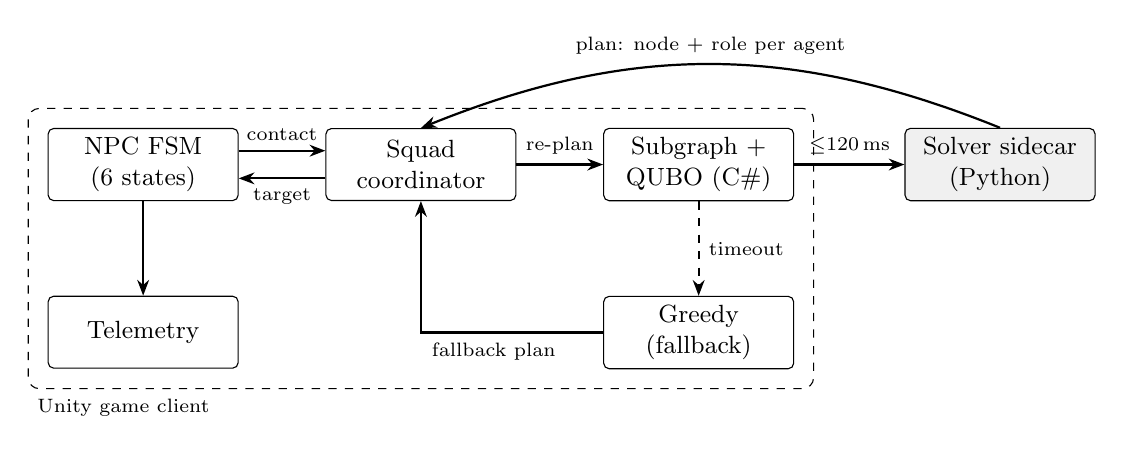
\begin{tikzpicture}[
  box/.style={draw, rounded corners=2pt, align=center, font=\small, minimum height=2.6em, text width=6.2em, fill=white},
  arr/.style={-{Stealth[length=2mm]}, thick},
  lab/.style={font=\scriptsize, align=center}]
\node[box] (fsm) {NPC FSM\\(6 states)};
\node[box, right=1.1cm of fsm] (coord) {Squad\\coordinator};
\node[box, right=1.1cm of coord] (qubo) {Subgraph +\\QUBO (C\#)};
\node[box, right=1.4cm of qubo, fill=black!6] (side) {Solver sidecar\\(Python)};
\node[box, below=1.2cm of fsm] (tele) {Telemetry};
\node[box, below=1.2cm of qubo] (greedy) {Greedy\\(fallback)};
\draw[arr] ([yshift=5pt]fsm.east) -- node[lab, above]{contact} ([yshift=5pt]coord.west);
\draw[arr] ([yshift=-5pt]coord.west) -- node[lab, below]{target} ([yshift=-5pt]fsm.east);
\draw[arr] (coord) -- node[lab, above]{re-plan} (qubo);
\draw[arr] (qubo) -- node[lab, above]{$\le$120\,ms} (side);
\draw[arr] (side.north) to[bend right=22] node[lab, above]{plan: node + role per agent} (coord.north);
\draw[arr, dashed] (qubo) -- node[lab, right]{timeout} (greedy);
\draw[arr] (greedy.west) -| node[lab, below, pos=.3]{fallback plan} (coord.south);
\draw[arr] (fsm) -- (tele);
\node[draw, dashed, rounded corners, fit=(fsm)(coord)(qubo)(greedy)(tele), inner sep=7pt,
  label={[font=\scriptsize, anchor=north west]south west:Unity game client}] {};
\end{tikzpicture}
\caption{Re-planning loop. A contact triggers a re-plan of the combat group; the QUBO is built in Unity and solved by the sidecar within the budget, otherwise by Greedy in process. The plan only sets each agent's destination and role; moving, shooting, and retreating stay with its FSM.}
\label{fig:architecture}
\end{figure}

Re-planning runs asynchronously under a coordination latency budget of 120\,ms, counted from the arrival of the request at the sidecar; one research solve runs at a time in a separate worker process, and the sidecar is started by the game on demand and exits with it. If the sidecar does not answer within the budget, Unity applies an in-process Greedy assignment as a fallback and records the reason, so gameplay never blocks on the solver. Re-planning is triggered by the first contact, by a significant move of the player, and by an agent dying or retreating, with a cooldown of 0.8\,s; a plan made for a player who has meanwhile moved away is discarded. Squads within radio range merge into one combat group of up to 8 agents, so that small camps are planned together. Only solvers that fit the budget are used during play; QAOA is evaluated offline. The web back end is not part of this gameplay loop.

The coordinator does not replace individual NPC behaviour. Each NPC runs the same six-state FSM (Figure~\ref{fig:fsm}); the plan only supplies the destination used by \textit{TakeCover} and the role that decides whether the agent holds that position. A boss is excluded from squad plans and chooses its own cover positions.

\begin{figure}[htbp]
\centering
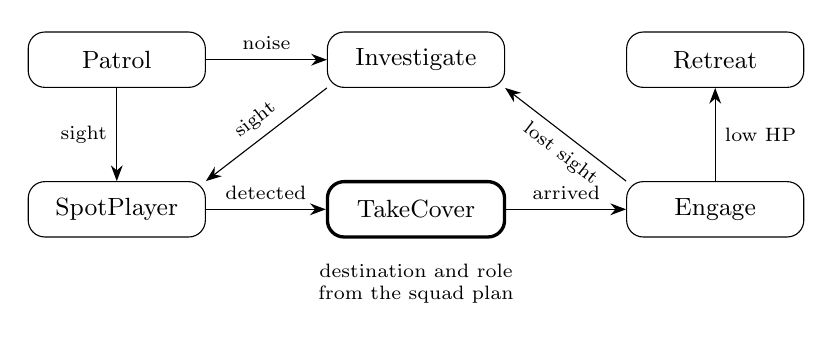
\begin{tikzpicture}[
  st/.style={draw, rounded corners=6pt, font=\small, minimum width=6.4em, minimum height=2em, fill=white},
  hot/.style={st, line width=1.2pt},
  arr/.style={-{Stealth[length=2mm]}},
  lab/.style={font=\scriptsize}]
\node[st]  (patrol)  at (0,0)      {Patrol};
\node[st]  (inv)     at (3.8,0)    {Investigate};
\node[st]  (retreat) at (7.6,0)    {Retreat};
\node[st]  (spot)    at (0,-1.9)   {SpotPlayer};
\node[hot] (cover)   at (3.8,-1.9) {TakeCover};
\node[st]  (engage)  at (7.6,-1.9) {Engage};
\draw[arr] (patrol) -- node[lab, above]{noise} (inv);
\draw[arr] (patrol) -- node[lab, left]{sight} (spot);
\draw[arr] (inv.south west) -- node[lab, above, sloped]{sight} (spot.north east);
\draw[arr] (spot) -- node[lab, above]{detected} (cover);
\draw[arr] (cover) -- node[lab, above]{arrived} (engage);
\draw[arr] (engage) -- node[lab, right]{low HP} (retreat);
\draw[arr] (engage.north west) -- node[lab, below, sloped, pos=.45]{lost sight} (inv.south east);
\node[font=\scriptsize, align=center, below=0.2cm of cover] {destination and role\\from the squad plan};
\end{tikzpicture}
\caption{The shared six-state NPC FSM. Only \textit{TakeCover} reads the coordinator's output.}
\label{fig:fsm}
\end{figure}

Supported solver modules include:

\begin{itemize}
\item Greedy (also the in-process fallback),
\item Greedy with local search, tabu search, and simulated annealing over assignments (SA-1h),
\item Genetic Algorithm,
\item Simulated Annealing over bits (dwave-neal),
\item PBIL (ablation of QIEA's Q-bit),
\item Simulated Quantum Annealing,
\item QIEA,
\item QAOA (offline, $\le 18$ variables),
\item exact enumeration, the set reduction with the Hungarian method, and branch and bound (reference only).
\end{itemize}

The common solver interface enables controlled experiments using identical QUBO instances.

% ------------------------------------------------------------
\subsection*{Content and Telemetry Platform}

The web platform is implemented with a ReactJS and Vite front end, an ASP.NET Core Web API back end with JWT-based role access, and a PostgreSQL database.

The platform allows authorized users to manage gameplay parameters such as:

\begin{itemize}
\item NPC health,
\item damage,
\item movement speed,
\item tactical weights,
\item QUBO penalty coefficients,
\item solver configuration.
\end{itemize}

Telemetry generated by game sessions is transmitted to an ingest API and stored for later analysis.

No directly identifying player information is required for the research dataset. Test sessions can instead be associated with randomized session identifiers.

% ============================================================
\section*{Experimental Design}

\subsection*{Benchmark Generation}

Because general-purpose optimization datasets do not directly represent ShadowVale tactical encounters, the project generates reproducible tactical benchmark instances.

Each instance contains:

\begin{itemize}
\item agent positions,
\item tactical points,
\item utility scores,
\item conflict relationships,
\item accessibility information.
\end{itemize}

Procedural generation uses fixed random seeds so that every solver receives exactly the same problem instances.

This allows direct algorithm comparison. The generated suites are complemented by instances recorded inside the game: every re-plan during the scripted replays writes the subgraph, agent and player nodes, weights, and seed, from which the benchmark rebuilds exactly the QUBO that Unity solved. To relate the results to established benchmarks, the same solvers are also run on the Quadratic Assignment Problem library QAPLIB \cite{Burkard1997} (gap to the published optimum) and on coordination instances drawn on Moving AI game maps \cite{Sturtevant2012}. Table~\ref{tab:suites} lists the suites of the official run.

\begin{table}[htbp]
\centering
\small
\begin{tabular}{lrrrrr}
\toprule
Suite & Nodes $N$ & Agents $A$ & Variables $n$ & Instances & Runs per solver \\
\midrule
small (exact optimum) & 6--10 & 2--3 & 12--30 & 180 & 5 \\
full (scalability) & 20--100 & 4--12 & 80--1{,}200 & 1{,}350 & 3 \\
game (recorded in play) & 19--24 & 2--8 & 44--184 & 4{,}549 (3{,}447 evaluated) & 3 \\
Moving AI maps & 16--24 & 4--8 & 80--192 & 342 & 3 \\
QAPLIB & 12--30 & 12--30 & 144--900 & 77 & 5 \\
\bottomrule
\end{tabular}
\caption{Benchmark suites of the official run exp-v2. Generated suites vary the chokepoint density over $\{0, 0.3, 0.6\}$ and use 30 seeds per cell (10 for small). The recorded game instances are those of exp-v1; a hashed quarter of them is the tuning split. Moving AI: combinations of 4 agents with fewer than 20 nodes do not occur, hence at least 80 variables. QAPLIB: every instance with $n\le30$ and a published solution.}
\label{tab:suites}
\end{table}

% ------------------------------------------------------------
\subsection*{Candidate Reduction}

The complete navigation graph may contain many nodes, but not every navigation node needs to become a QUBO variable.

In ShadowVale the reduction is spatial: at most 24 nodes enter the QUBO, the agents' own nodes and the nodes nearest to the player, whatever the size of the map graph (451 nodes on Map 1). Therefore

$$
n = A\,|V| \le 8 \times 24 = 192
$$

in play. A 2-agent, 6-node instance has $n=12$ variables; a statevector simulator stores $2^{12}$ amplitudes and its $6\cdot5=30$ feasible assignments (one node per agent, no node shared) are enumerated instantly. A 6-agent group over 24 nodes has $n=144$ variables and $24!/18! \approx 9.7 \times 10^{7}$ feasible assignments, beyond QAOA simulation and exhaustive search within a real-time budget, although the set reduction needs only $\binom{24}{6}=134{,}596$ node sets. This second regime is where heuristic, simulated-quantum, and quantum-inspired solvers must be compared.

Candidate reduction is essential for maintaining computational feasibility.

% ------------------------------------------------------------
\subsection*{QAOA Experimental Scope}

Classical simulation of a generic quantum state may require resources that grow exponentially with the number of qubits.

Consequently, QAOA is evaluated primarily on small QUBO instances.

The benchmark is divided into two regimes.

\textbf{Common Solver Regime:}

Small instances with $n \le 18$ binary variables are solved by all methods:

$$
\text{Greedy},
\text{GA},
\text{SA},
\text{QIEA},
\text{SQA},
\text{QAOA}.
$$

These instances allow direct comparison with an exact optimum whenever computationally feasible.

\textbf{Scalability Regime:}

Larger instances, up to 12 agents over 100 nodes ($n \le 1{,}200$), are evaluated using:

$$
\text{Greedy},
\text{GA},
\text{SA},
\text{QIEA},
\text{SQA}.
$$

QAOA results are not extrapolated beyond the simulator's practical resource limits.

This separation prevents simulator limitations from being incorrectly interpreted as limitations of the mathematical QUBO formulation itself.

% ------------------------------------------------------------
\subsection*{Experimental Protocol}

For each problem size, 30 instances are generated from fixed seeds per density, and every stochastic solver is run 3--5 times per instance with independent solver seeds (Table~\ref{tab:suites}). All solvers are compared at the same wall-clock budget as in play, 120\,ms on one CPU thread, on one machine and without the game running; QAPLIB is additionally run at 1{,}000\,ms. The number of energy evaluations is logged per run. Before the official run, GA, SA, SQA, and QIEA were tuned with the same effort (30 configurations each, including the default) on a separate tuning split (seeds 901+ and a hashed quarter of the recorded instances), which the evaluation excludes. QAOA is run with the same 120\,ms budget but exceeds it from 16 variables; it is additionally studied without any budget, reading the probability of the optimum directly from the statevector and comparing it with uniform random sampling.

Results are summarized by the mean gap and the share of runs that reach the reference, and latency reports the median and the 95th percentile. For each pair of solvers the repeats of an instance are averaged first, so that the instance is the unit of analysis, and the Wilcoxon signed-rank test is applied over instances, with Holm correction over the pairs of each suite \cite{Holm1979}; differences are reported in percentage points with bootstrap 95\,\% confidence intervals, and differences below 0.1 percentage point are treated as practically negligible however small their $p$-value. The number of energy evaluations per run is reported next to the latency. Every result row records the commit it ran on, and only clean, tagged commits were used.

% ============================================================
\section*{Evaluation Metrics}

\subsection*{Solution Quality}

For sufficiently small instances, the global optimum

$$
E^*
$$

is obtained using exhaustive enumeration or another exact method.

For an algorithm returning energy

$$
E_{\text{alg}},
$$

the relative optimality gap is defined as

$$
G
=
\frac{E_{\text{alg}}-E^*}
{\max(1,|E^*|)}.
$$

A smaller value indicates a solution closer to the known optimum.

If

$$
G=0,
$$

the algorithm has found an optimal solution.

This metric is preferred over a simple approximation ratio because the QUBO objective may contain negative energies.

Energies include the constant $M|I|$ produced by expanding the assignment penalty, so that on every feasible assignment $E=-F$ and the gap equals $(F^*-F)/|F^*|$. Every reported output is feasible (after the repair described below), so the gap is always defined. $E^*$ is the proven optimum (enumeration, set reduction or branch and bound) wherever one is available, which covers all recorded game instances, the small suite, the Moving AI instances and the full-suite instances with at most $5\times10^6$ node sets; otherwise it is the best of two independent 2\,s runs (tabu search and GA) that take no part in the comparison, so that the reference is not produced by the runs being ranked. A 120\,ms run that beats this reference gets a negative gap. The approximation ratio of the first version is no longer used.

% ------------------------------------------------------------
\subsection*{Feasibility Rate}

A returned solution is feasible when every participating agent has exactly one position and no position is shared, i.e.\ when it encodes an injective assignment:

$$
\sum_{r\in R_i}x_{i,r}=1\;\;\forall i, \qquad \sum_{i}x_{i,r}\le 1\;\;\forall r .
$$

SA, SQA and QAOA return raw bit vectors; an infeasible one is repaired by keeping, per agent, its set bit of lowest marginal energy and giving agents without a position, or with a taken one, the cheapest free position. The repair costs about as much as Greedy and is not included in the reported latency. Feasibility before repair (\emph{raw feasibility}) is reported for every solver; GA, tabu search and the local searches are feasible by construction; QIEA and PBIL repair every sample.

Raw feasibility rate is calculated as

$$
\text{Feasibility Rate}
=
\frac{\text{Number of outputs feasible before repair}}
{\text{Total solver runs}}.
$$

This metric is particularly useful for evaluating whether the selected penalty parameter $M$ is sufficiently large.

% ------------------------------------------------------------
\subsection*{Wall-Clock Latency}

Latency is measured using wall-clock time and divided into:

\begin{itemize}
\item QUBO construction time,
\item solver execution time,
\item post-processing time,
\item total coordination latency.
\end{itemize}

Because stochastic algorithms may have long-tail behavior, both median latency and high-percentile latency such as the 95th percentile are reported where possible.

% ------------------------------------------------------------
\subsection*{Scalability}

Scalability experiments vary:

\begin{itemize}
\item number of NPCs $N$,
\item candidate positions per NPC $K$,
\item total number of QUBO variables $n$,
\item number of pairwise conflict terms.
\end{itemize}

The objective is to determine how rapidly solution quality and latency change as tactical complexity increases.

% ============================================================
\section*{Gameplay Telemetry Evaluation}

Optimization quality alone does not establish that an algorithm produces better gameplay.

Therefore, mathematical results are evaluated together with game telemetry.

To make gameplay measurements repeatable, a scripted player agent replays fixed escape policies on the same encounters and seeds for every solver. Three exploit bots attack the same camp of Map 1: \textit{same\_route} always crosses the camp on the same path and keeps running, \textit{same\_bush} shows itself and then hides in the same bush, and \textit{stone\_lure} throws a stone to one side and sneaks past on the other. Each bot's difficulty knob was calibrated on Greedy (seeds 500+, 10 seeds per value, coarse then fine grid) on the final build to a capture rate near 50\,\%, before any solver was compared. Every variant plays the same 100 seeds per bot (1000+) at a fixed 30\,fps step; because the fixed step runs faster than real time, the game waits for each solve and applies the plan after its real latency in game time (lockstep), so remote solvers are not penalised by the speed-up. A control variant without coordination (``none'': radio alerts only, every agent on its own FSM) separates the effect of coordinating from the choice of solver. Coverage, escape time, and capture rate can then be compared across solvers without variation in human skill. The human pilot study described below complements these scripted runs.

The following gameplay metrics are collected.

\subsection*{Tactical Coverage Score}

The tactical coverage (coordination) score of a plan is the share of the subgraph's escape nodes that are visible from at least one of the plan's positions; a run reports the mean over its re-plans. It is the escape-route component of the objective, measured on the plans actually applied.

% ------------------------------------------------------------
\subsection*{Player Escape Time}

Escape time is the duration of an encounter that ends with the player escaping: from the first contact to the moment the last guard lost the player, provided no guard regains contact within the following 2\,s.

This metric provides an observable gameplay consequence of tactical coordination.

% ------------------------------------------------------------
\subsection*{Capture or Combat Success Rate}

Capture rate is the share of runs in which the player is killed while the squad is engaged. Captures are compared between variants on paired seeds with the exact McNemar test (Holm-corrected over the comparisons against Greedy and against \emph{none}); escape time and coverage are compared with the Wilcoxon signed-rank test on paired seeds. Capture rates are reported with Wilson 95\,\% intervals.

A higher capture rate is not automatically interpreted as better gameplay, because excessive difficulty may reduce fairness.

% ============================================================
\section*{Results}

All numbers below come from the official run exp-v2 (solver commit \texttt{a12809f}, tag exp-v2; game commit \texttt{525ded1} for the replay), which repeats exp-v1 after the review of the first version and adds the solvers, references and statistics it asked for. Raw CSV and JSONL files, the tuning logs and \texttt{analysis.txt}, which lists every number quoted here, are in \texttt{experiments/results/exp-v2}. Every returned answer is a feasible assignment; for SA, SQA and QAOA this is after the repair described in the metrics section.

\subsection*{Solution Quality and Latency on In-Game Problems}

Table~\ref{tab:solvers} reports every solver at the 120\,ms budget. The set reduction proves the optimum of all 3{,}447 evaluated game instances (the first version could prove 2{,}529 of them), so every game-instance gap is to a proven optimum.

\begin{table}[htbp]
\centering
\resizebox{\linewidth}{!}{\begin{tabular}{lrrrrrrrrr}
\toprule
 & \multicolumn{5}{c}{Recorded game instances} & Full & Moving & \multicolumn{2}{c}{QAPLIB} \\
\cmidrule(lr){2-6}\cmidrule(lr){7-7}\cmidrule(lr){8-8}\cmidrule(lr){9-10}
Solver & gap & opt. & p50 & evals & raw & gap & AI gap & 120\,ms & 1\,s \\
 & \% & \% & ms & & feas.\,\% & \% & \% & \% & \% \\
\midrule
Greedy & 2.76 & 39.5 & 0.13 & -- & 100 & 8.18 & 10.20 & 73.1 & 73.1 \\
Greedy+LS & 0.27 & 74.7 & 0.40 & 144 & 100 & 1.32 & 0.50 & 15.3 & 10.4 \\
Tabu & 0.000 & 99.9 & 96.1 & 77{,}550 & 100 & 0.78 & 0.00 & 7.5 & 1.5 \\
GA & 0.11 & 78.2 & 96.1 & 1{,}966 & 100 & 2.70 & 0.56 & 19.7 & 9.5 \\
SA (bits) & 3.91 & 34.7 & 98.9 & 136 & 100 & 29.52 & 9.06 & 66.1 & 46.6 \\
SA-1h & 0.087 & 80.3 & 95.9 & 2{,}854 & 100 & 2.75 & 0.50 & 16.1 & 5.2 \\
PBIL & 0.036 & 90.4 & 96.1 & 1{,}474 & 15 & 2.14 & 0.86 & 28.5 & 13.1 \\
SQA & 4.10 & 33.0 & 84.0 & 640 & 63 & 32.30 & 9.76 & 92.2 & 63.9 \\
QIEA & 0.11 & 82.1 & 96.1 & 1{,}028 & 0 & 2.19 & 2.57 & 26.4 & 14.8 \\
\bottomrule
\end{tabular}
}
\caption{All solvers at the 120\,ms budget. Gap: mean optimality gap per instance (repeats averaged first). Opt.: share of runs at the proven optimum. p50: median latency. Evals: median number of candidate evaluations per run (moves for Greedy+LS, tabu search and SA-1h; samples otherwise). Raw feas.: share of the solver's own samples that were valid assignments before repair. Full: gap to the proven optimum or to an independent 2\,s reference. QAPLIB: gap to the published optimum (76 of the 77 instances; one has optimum 0).}
\label{tab:solvers}
\end{table}

Tabu search finds the optimum in 99.9\,\% of the runs on game instances. Greedy is 2.76\,\% from the optimum on average (optimal in 39.5\,\% of the runs); a local search on top of it (Greedy+LS, median 0.40\,ms, 95th percentile 1.34\,ms) reduces this to 0.27\,\%, which closes 90\,\% of the gap that the 120\,ms methods close. PBIL (0.036\,\%), SA-1h (0.087\,\%), GA (0.107\,\%) and QIEA (0.108\,\%) lie between. QIEA and GA are statistically indistinguishable (difference $+0.001$ percentage points, 95\,\% CI $[-0.009, 0.010]$, $p=0.42$); the advantage of QIEA reported in the first version (0.04 vs.\ 0.09\,\%) came from scoring only the 2{,}529 instances whose optimum the branch and bound could prove. PBIL is ahead of QIEA by 0.07 percentage points; the difference is statistically clear ($p_{\text{Holm}}<10^{-70}$) but practically negligible. The bit-flip samplers SA and SQA are worse than Greedy (3.9 and 4.1\,\%) although they spend the same time; only 63\,\% of SQA's samples are valid assignments, and QIEA's and PBIL's raw bit samples almost never are before repair (0 and 15\,\%).

\subsection*{Scalability}

Figures~\ref{fig:quality} and \ref{fig:latency} show the full suite (1{,}350 instances up to 1{,}200 variables) separately by number of agents and number of nodes, with bootstrap confidence intervals, as the review requested. The reference is a proven optimum for the 630 instances with at most $5\times10^6$ node sets and the better of two independent 2\,s runs (tabu search and GA) for the other 720; no 120\,ms run beat that reference. Tabu search is the most accurate (0.78\,\% on average, at the reference in 88\,\% of the runs), followed by Greedy+LS (1.32\,\%), PBIL (2.14\,\%), QIEA (2.19\,\%, not different from PBIL, $p=0.27$), GA (2.70\,\%) and SA-1h (2.75\,\%); Greedy stays near 8\,\% at every size. With 4 agents tabu search is exact up to 100 nodes; with 12 agents over 100 nodes (1{,}200 variables) every method ends near Greedy (9.0--9.6\,\%), because one iteration of our Python implementations no longer fits many times into 120\,ms. SA and SQA degrade from about 9\,\% at 80 variables to 36--57\,\%, and bit-flip SA exceeds the budget from about 600 variables because dwave-neal's batches cannot be interrupted. Re-measured one process at a time on the idle machine (90 instances of the full suite and 415 game instances), no solver except bit-flip SA (34\,\% of the full-suite runs) and SQA (1\,\%) exceeded the budget; Greedy took at most 53\,ms and Greedy+LS 63\,ms at 1{,}200 variables, and on game instances Greedy+LS took at most 0.8\,ms. The latencies of the main runs, which ran as up to seven concurrent processes, are slightly higher.

\begin{figure}[htbp]
\centering
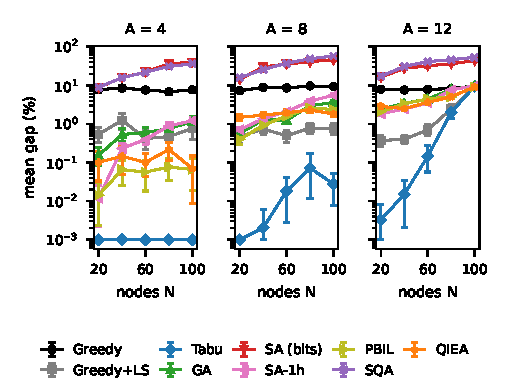
\includegraphics[width=\linewidth]{figures/full_quality.pdf}
\caption{Full suite: mean gap per instance by number of nodes, one panel per number of agents (log scale; error bars: bootstrap 95\,\% CI; a gap of 0 is drawn at $10^{-3}$\,\%).}
\label{fig:quality}
\end{figure}

\begin{figure}[htbp]
\centering
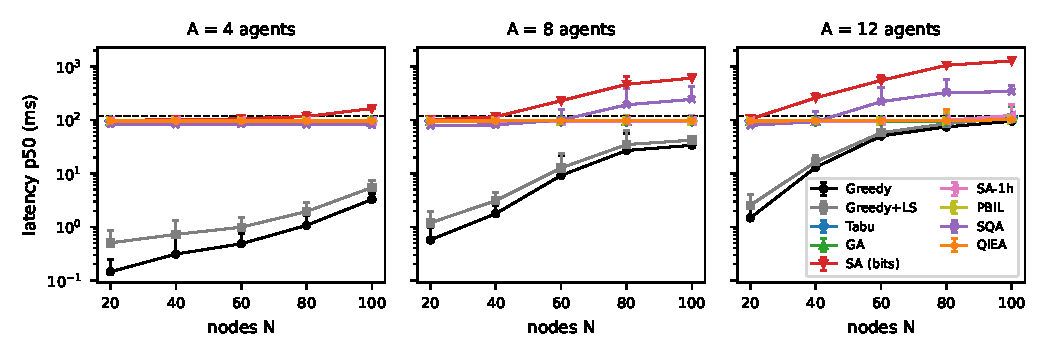
\includegraphics[width=\linewidth]{figures/full_latency.pdf}
\caption{Full suite: median latency by number of nodes, one panel per number of agents; error bars up to the 95th percentile; dashed line, the 120\,ms budget.}
\label{fig:latency}
\end{figure}

\subsection*{Public Datasets}

On the Moving AI coordination instances (342, all with a proven optimum) the ranking of the game instances holds: tabu search 0.002\,\%, SA-1h and Greedy+LS 0.50\,\%, GA 0.56\,\%, PBIL 0.86\,\%, QIEA 2.57\,\%, and the bit-flip samplers about 9\,\%, close to Greedy (10.2\,\%). QAPLIB is much harder for every method: at 120\,ms tabu search is 7.5\,\% from the published optimum, against 19.7\,\% for GA and 26.4\,\% for QIEA, and with 1\,s it reaches 1.5\,\% (SA-1h 5.2\,\%, GA 9.5\,\%, QIEA 14.8\,\%, SA 46.6\,\%, SQA 63.9\,\%). GA, the strongest classical method of the first version, is therefore not the strongest classical baseline.

\subsection*{QAOA without the Shot and Budget Confounds}

On the small suite (180 instances of 12--30 variables, optimum by enumeration), tabu search and SA-1h reach the optimum in every run, QIEA, PBIL and GA in 98--100\,\% of the runs (mean gap at most 0.01\,\%), bit-flip SA and SQA in 95 and 92\,\%, Greedy+LS in 81\,\% and Greedy in 29\,\% (gap 4.4\,\%). QAOA under the 120\,ms budget behaves as in the first version: at 12 variables its best measured bit string is optimal in 94\,\% of the runs (median 103\,ms), at 16 and 18 variables in 7.3 and 6.0\,\% of the runs, with only 30 and 16\,\% of the returned bit strings valid before repair, and a median latency of 173 and 568\,ms, above the budget. These numbers mix the circuit with the number of shots and the time limit, which the following study separates.

Table~\ref{tab:qaoa} reads QAOA from the statevector, with angles optimized without a time limit, so that neither the budget nor the number of shots affects the result, and compares it with uniform random sampling.

\begin{table}[htbp]
\centering
\begin{tabular}{rrlrrrrr}
\toprule
$n$ & $A{\times}|V|$ & mixer & $P_\text{valid}$ & $P_\text{opt}$ & $P_\text{opt}$/uniform & hit$_{512}$ & uniform hit$_{512}$ \\
\midrule
12 & 2$\times$6 & X & 0.35 & 0.0144 & 0.39 & 1.00 & 1.00 \\
12 & 2$\times$6 & XY & 1.00 & 0.0519 & 1.13 & 1.00 & 1.00 \\
16 & 2$\times$8 & X & 0.34 & 0.0075 & 0.35 & 0.97 & 1.00 \\
16 & 2$\times$8 & XY & 0.97 & 0.0243 & 0.97 & 0.99 & 1.00 \\
18 & 3$\times$6 & X & 0.17 & 0.0018 & 0.19 & 0.59 & 0.99 \\
18 & 3$\times$6 & XY & 0.95 & 0.0103 & 1.14 & 0.98 & 0.99 \\
20 & 2$\times$10 & XY & 0.97 & 0.0130 & 0.95 & 0.90 & 1.00 \\
24 & 3$\times$8 & XY & 0.85 & 0.0032 & 0.60 & 0.67 & 0.81 \\
30 & 3$\times$10 & XY & 0.85 & 0.0013 & 0.72 & 0.44 & 0.56 \\
40 & 4$\times$10 & XY & 0.72 & 0.0002 & 0.92 & 0.11 & 0.14 \\
40 & 5$\times$8 & XY & 0.41 & 0.0001 & 0.13 & 0.04 & 0.11 \\
48 & 4$\times$12 & XY & 0.83 & 0.0001 & 0.56 & 0.05 & 0.07 \\
\bottomrule
\end{tabular}

\caption{QAOA at depth $p=3$, means over instances (30 per size; 20 and 10 for the two largest). $P_\text{valid}$, $P_\text{opt}$: probability of measuring a valid assignment, an optimal one. $P_\text{opt}$/uniform: median ratio to sampling valid assignments uniformly. hit$_{512}$: probability that 512 shots contain the optimum, for QAOA and for 512 uniformly drawn valid assignments. X: standard mixer; XY: ring-XY mixer, simulated in the one-hot sector.}
\label{tab:qaoa}
\end{table}

With the standard mixer at most 35\,\% of the probability lies on valid assignments, and the optimum receives only 0.19--0.39 times the probability that uniform sampling of valid assignments gives it; 512 shots contain the optimum in 59\,\% of the 18-variable instances, against 99\,\% for 512 uniformly drawn valid assignments. QAOA is far better than uniform sampling of \emph{bit strings} (whose 512 shots contain the optimum in 13\,\% of the 12-variable and 0.2\,\% of the 18-variable instances), which is what made it look strong in the first version, but that is not the relevant baseline: with 512 shots at 12 variables, almost any sampler finds the optimum. The constraint-preserving XY ansatz \cite{Hadfield2019,Wang2020XY} keeps 41--100\,\% of the probability on assignments without clashes and could be simulated up to 48 variables, yet its probability of the optimum stays between 0.13 and 1.14 times the uniform one (median per size), and its 512-shot hit rate never exceeds that of uniform valid sampling. These conclusions concern our simulation (depth $p\le3$, grid plus Nelder--Mead angle search), not QAOA in general.

\subsection*{Gameplay Effect of Coordination}

Figure~\ref{fig:replay} and Table~\ref{tab:replay} summarize 1{,}800 replays on the final build (3 bots $\times$ 6 variants $\times$ 100 paired seeds, two Unity projects at the same commit, each with its own sidecar). No re-plan fell back to Greedy, so every planned variant was measured with its own solver (in the first version 0--17\,\% of the re-plans of SA and SQA had fallen back).

\begin{figure}[htbp]
\centering
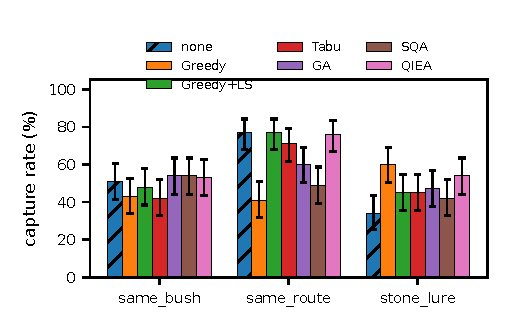
\includegraphics[width=0.75\linewidth]{figures/replay_capture.pdf}
\caption{Capture rate by exploit bot and coordination variant on the final build, 100 paired seeds each, with 95\,\% Wilson intervals. Hatched: no coordination (FSM only).}
\label{fig:replay}
\end{figure}

\begin{table}[htbp]
\centering
\begin{tabular}{lrrrrrrr}
\toprule
Bot & none & Greedy & Greedy+LS & Tabu & GA & SQA & QIEA \\
\midrule
same\_bush & 51 {\scriptsize[41,61]} & 43 {\scriptsize[34,53]} & 48 {\scriptsize[38,58]} & 42 {\scriptsize[33,52]} & 54 {\scriptsize[44,63]} & 54 {\scriptsize[44,63]} & 53 {\scriptsize[43,62]} \\
same\_route & 77 {\scriptsize[68,84]} & 41 {\scriptsize[32,51]} & 77 {\scriptsize[68,84]} & 71 {\scriptsize[61,79]} & 60 {\scriptsize[50,69]} & 49 {\scriptsize[39,59]} & 76 {\scriptsize[67,83]} \\
stone\_lure & 34 {\scriptsize[25,44]} & 60 {\scriptsize[50,69]} & 45 {\scriptsize[36,55]} & 45 {\scriptsize[36,55]} & 47 {\scriptsize[38,57]} & 42 {\scriptsize[33,52]} & 54 {\scriptsize[44,63]} \\
\midrule
all bots & 54 {\scriptsize[48,60]} & 48 {\scriptsize[42,54]} & 57 {\scriptsize[51,62]} & 53 {\scriptsize[47,58]} & 54 {\scriptsize[48,59]} & 48 {\scriptsize[43,54]} & 61 {\scriptsize[55,66]} \\
\bottomrule
\end{tabular}

\caption{Capture rate (\%) per bot and variant with Wilson 95\,\% intervals (100 paired seeds per cell).}
\label{tab:replay}
\end{table}

The choice of solver changes play, but not in one direction. Against \textit{same\_route}, Greedy+LS and QIEA capture the bot in 77 and 76\,\% of the seeds against 41\,\% for Greedy (exact McNemar test on paired seeds, $p_\text{Holm}<0.001$), as often as guards without plans (77\,\%, which captured far more than Greedy, $p_\text{Holm}<10^{-6}$); GA (60\,\%) and SQA (49\,\%) lie between. Against \textit{stone\_lure}, Greedy captures most (60\,\%) and the uncoordinated squad least (34\,\%, $p_\text{Holm}=0.003$): the plan keeps guards on the escape routes instead of all following the stone; QIEA also beats \textit{none} (54\,\%, $p_\text{Holm}=0.023$). Against \textit{same\_bush} no variant differs from Greedy or from \textit{none} (43--54\,\%). Pooled over the three bots, QIEA captures more than Greedy (61 vs.\ 48\,\%, $p_\text{Holm}=0.015$), but not significantly more than no coordination (54\,\%, $p_\text{Holm}=0.42$); no other variant differs significantly from Greedy.

The tactical coverage of the applied plans hardly differs between solvers (0.65--0.73 of the escape nodes in view; differences of at most 0.04, significant only because they are paired), although their objective values differ by several percent. Greedy's squads keep an escaping player in the encounter longer than squads without plans (mean escape time 7.4 vs.\ 4.8\,s, $p_\text{Holm}<10^{-6}$; GA and SQA also do, Greedy+LS and QIEA not significantly); between solvers, Greedy+LS and QIEA give shorter escapes than Greedy (5.6 and 5.1\,s, $p_\text{Holm}=0.02$ and $0.04$), partly because they capture the fleeing bot before it escapes. Plan quality is therefore at best loosely related to capture: against \textit{same\_route}, Greedy's plans send guards to positions from which the fleeing bot escapes, while the near-optimal plans of Greedy+LS and QIEA catch it as often as guards that simply chase; against the decoy the order is reversed. The hand-set weights of the objective were never tuned against such outcomes.

\subsection*{Answers to the Research Questions}

\begin{itemize}
\item \textbf{RQ1.} Squad assignment is expressed as a QUBO with five tactical terms and a penalty weight under which every global minimum is feasible (proof sketch and exhaustive tests); it is built identically in C\# and Python. Because only travel cost depends on the agent, the exact problem reduces to choosing a node set plus a linear assignment, which proves game-size optima in about 0.1\,s.
\item \textbf{RQ2.} Under equal 120\,ms budgets the strongest method is classical: tabu search (optimal in 99.9\,\% of game runs; 1.5\,\% from the QAPLIB optimum at 1\,s). Greedy with local search reaches 0.27\,\% in under 2\,ms. QIEA is as accurate as GA on game instances and no more accurate than PBIL except on QAPLIB at 120\,ms, so its Q-bit representation is not what makes it work. Bit-flip SA and SQA are worse than Greedy; annealing over assignments (SA-1h) is not, so their weakness lies in the encoding. Feasibility of the returned answers is 100\,\% after repair for all solvers; raw feasibility separates them.
\item \textbf{RQ3.} Greedy's quality is independent of size; tabu search is exact with 4 agents up to 100 nodes; with 12 agents over 100 nodes, all 120\,ms methods fall back to Greedy's level in our Python implementations; bit-flip SA and SQA lose accuracy fastest and exceed the budget.
\item \textbf{RQ4.} Standard QAOA simulation stays within the budget only at 12 variables and is refused beyond 18 by our simulator; read from the statevector, neither the standard nor the XY ansatz produces the optimum more often than uniform sampling of valid assignments, at any size we simulated (up to 48 variables). In-game re-plans have 44--184 variables, or $|V|\le24$ binary decisions in the reduced formulation.
\item \textbf{RQ5.} Yes, but not in one direction. With 100 paired seeds per cell, the solver changed capture rates by up to 36 points against one exploit (Greedy 41\,\% vs.\ Greedy+LS 77\,\% and QIEA 76\,\%), was reversed against another (Greedy highest), and made no difference against the third; whether the squad coordinates at all mattered as much (34 vs.\ 60\,\% against the decoy). Better optimization of the current objective is not a reliable proxy for a stronger opponent.
\end{itemize}



% ============================================================
\section*{Pilot Player Study}

A small controlled playtest was designed to investigate whether different coordination algorithms are perceptible to human players. It was not conducted within this project, and no human-player results are reported; the design below is left for future work.

Participants play comparable encounters under at least two conditions:

\begin{itemize}
\item classical Greedy coordination,
\item optimization-based coordination using the best-performing candidate solver from offline experiments.
\end{itemize}

Encounter order should be counterbalanced where possible to reduce learning effects.

Gameplay telemetry is collected together with a short post-session questionnaire measuring perceived:

\begin{itemize}
\item predictability,
\item coordination,
\item difficulty,
\item fairness.
\end{itemize}

With approximately five participants, such an experiment would be a pilot usability study whose results are descriptive and not statistically representative of the general player population.

% ============================================================
\section*{Threats to Validity and Limitations}

Several limitations must be considered when interpreting the results.

First, QAOA is executed on a classical simulator rather than physical quantum hardware.

Therefore, simulator latency cannot be interpreted as the latency of a future fault-tolerant quantum computer.

Second, QAOA simulation scales poorly with the number of qubits. The algorithm is therefore evaluated on smaller instances than some classical and quantum-inspired methods.

Third, QIEA and SQA are executed on classical hardware. Their use of quantum-inspired or quantum-simulation concepts does not imply quantum computational advantage.

Fourth, gameplay behavior depends not only on assignment quality but also on navigation, animation, weapon mechanics, level design, and player skill.

Consequently, telemetry differences cannot automatically be attributed exclusively to the optimization algorithm.

Fifth, a small human playtest provides exploratory evidence only.

Sixth, the replay measures one camp of one map against three scripted strategies, and absolute capture rates depend on the FSM, weapon and boss tuning of the build it ran on. The replay of the first version predated several gameplay changes (fight-first FSM rule, hit chance, health regeneration, a shorter reinforcement range); it was repeated on the final build (exp-v2) after recalibrating the bots, and only the repeated results are reported.

Seventh, all solvers were given a single 120\,ms wall-clock budget on one machine, and they are Python implementations of different efficiency (dwave-neal is compiled, the others use numpy), so wall-clock comparisons mix algorithm and implementation; evaluations per run are reported for this reason. A different budget or a faster implementation could change the ranking, as the QAPLIB run at 1{,}000\,ms shows. The offline exp-v2 runs were executed as several concurrent single-threaded processes on a 10-core CPU.

Eighth, the tactical weights $(1, 0.5, 1, 0.5, 0.1)$ were set by hand and were not tuned against gameplay outcomes; no sensitivity analysis was performed. A solver that is closer to the optimum of this objective is not necessarily a better opponent.

Finally, the proposed QUBO formulation is domain-specific. Additional evaluation would be required before claiming that it generalizes to other games or real-world multi-agent systems.

% ============================================================
\section*{Contributions}

The research provides four contributions.

First, the project applies the standard penalty-based QUBO encoding of assignment problems \cite{Glover2019} to multi-agent tactical assignment in a real-time game environment, contributing domain-specific tactical utility and conflict terms together with an explicit bound for the constraint penalty.

The formulation combines tactical utility, spatial conflict penalties, and agent-assignment constraints in a single optimization objective.

Second, the project provides an experimental comparison between quantum, simulated-quantum, quantum-inspired, and classical optimization methods under identical tactical problem instances.

The study does not assume in advance that a particular solver will outperform the others.

Instead, the objective is to identify the conditions under which each solver provides a useful trade-off between solution quality and computational cost.

Third, the project investigates the practical scalability boundary of QAOA simulation for tactical QUBO problems and compares this boundary with classical and quantum-inspired approaches.

Fourth, ShadowVale integrates optimization experiments with gameplay telemetry.

This enables the project to investigate whether mathematical improvements in tactical assignment correspond to observable differences in player interaction.

The implementation, benchmark generator, instances, tuning logs and raw results are released (\url{https://github.com/anhttse184743/shadowvale-solver/tree/exp-v2}, tag exp-v2), so the system can serve as a reproducible testbed for future research in optimization-based Game AI.

% ============================================================
\section*{Conclusion}

ShadowVale studies multi-agent tactical coordination as a combinatorial optimization problem rather than relying exclusively on handcrafted squad behavior.

By representing tactical assignment using QUBO, multiple competing requirements---including tactical utility, assignment feasibility, and spatial redundancy---can be expressed within a common mathematical objective.

The architecture supports multiple interchangeable solvers, including QAOA, Simulated Quantum Annealing, QIEA, Simulated Annealing, a Genetic Algorithm, and Greedy Assignment, with exact solvers as references.

The experiments answered three questions: solution quality, computational feasibility, and gameplay impact. Within a 120\,ms budget the best method is classical: tabu search is optimal in 99.9\,\% of in-game re-plans, and a millisecond of local search brings Greedy within 0.27\,\% of the optimum, which makes it the natural in-game fallback. The quantum-inspired QIEA is as accurate as a genetic algorithm and as PBIL without Q-bits; simulated quantum annealing does not outperform classical annealing, and both lose to Greedy when they flip raw bits of the one-hot encoding; and simulated QAOA does not produce the optimum more often than uniform sampling of valid assignments. Because only travel cost depends on the agent, the exact optimum of a game-size re-plan can be proven in about 0.1\,s. In play, the solver changed capture rates against some exploits but not consistently, and coordinating at all mattered as much as the solver. At this scale, cheap classical methods are sufficient; the quantum and quantum-inspired methods studied here show no advantage.

Rather than assuming quantum or quantum-inspired methods are superior, the research determined empirically their strengths, limitations, and practical operating ranges.

The resulting framework contributes an optimization-oriented perspective to Game AI and provides a foundation for studying more complex multi-agent tactical systems in future work.

% ============================================================
\begin{thebibliography}{99}

\bibitem{Farhi2014}
E. Farhi, J. Goldstone, and S. Gutmann,
``A Quantum Approximate Optimization Algorithm,''
arXiv:1411.4028, 2014.

\bibitem{Lucas2014}
A. Lucas,
``Ising formulations of many NP problems,''
\textit{Frontiers in Physics},
vol. 2, 2014.

\bibitem{HanKim2002}
K.-H. Han and J.-H. Kim,
``Quantum-Inspired Evolutionary Algorithm for a Class of Combinatorial Optimization,''
\textit{IEEE Transactions on Evolutionary Computation},
vol. 6, no. 6, pp. 580--593, 2002.

\bibitem{Sharon2015}
G. Sharon, R. Stern, A. Felner, and N. R. Sturtevant,
``Conflict-Based Search for Optimal Multi-Agent Pathfinding,''
\textit{Artificial Intelligence},
vol. 219, pp. 40--66, 2015.

\bibitem{Barkoutsos2020}
P. K. Barkoutsos et al.,
``Improving Variational Quantum Optimization using CVaR,''
\textit{Quantum},
vol. 4, p. 256, 2020.

\bibitem{QiskitAlgorithms}
Qiskit Community,
``Qiskit Algorithms: Quantum Approximate Optimization Algorithm (QAOA),''
Qiskit Algorithms documentation, 2024. \url{https://qiskit-community.github.io/qiskit-algorithms/}.

\bibitem{DWaveSamplers}
D-Wave Systems,
``dwave-neal: simulated annealing sampler,'' version 0.6.0, 2024. \url{https://github.com/dwavesystems/dwave-neal}.

\bibitem{Glover1989}
F. Glover,
``Tabu Search---Part I,''
\textit{ORSA Journal on Computing}, vol. 1, no. 3, pp. 190--206, 1989.

\bibitem{Taillard1991}
\'E. Taillard,
``Robust taboo search for the quadratic assignment problem,''
\textit{Parallel Computing}, vol. 17, no. 4--5, pp. 443--455, 1991.

\bibitem{Baluja1994}
S. Baluja,
``Population-Based Incremental Learning: A Method for Integrating Genetic Search Based Function Optimization and Competitive Learning,''
Technical Report CMU-CS-94-163, Carnegie Mellon University, 1994.

\bibitem{Hadfield2019}
S. Hadfield, Z. Wang, B. O'Gorman, E. G. Rieffel, D. Venturelli, and R. Biswas,
``From the Quantum Approximate Optimization Algorithm to a Quantum Alternating Operator Ansatz,''
\textit{Algorithms}, vol. 12, no. 2, p. 34, 2019.

\bibitem{Wang2020XY}
Z. Wang, N. C. Rubin, J. M. Dominy, and E. G. Rieffel,
``XY mixers: Analytical and numerical results for the quantum alternating operator ansatz,''
\textit{Physical Review A}, vol. 101, no. 1, 012320, 2020.

\bibitem{Kuhn1955}
H. W. Kuhn,
``The Hungarian method for the assignment problem,''
\textit{Naval Research Logistics Quarterly}, vol. 2, no. 1--2, pp. 83--97, 1955.

\bibitem{Ahuja2007}
R. K. Ahuja, A. Kumar, K. C. Jha, and J. B. Orlin,
``Exact and heuristic algorithms for the weapon-target assignment problem,''
\textit{Operations Research}, vol. 55, no. 6, pp. 1136--1146, 2007.

\bibitem{Gerkey2004}
B. P. Gerkey and M. J. Matari\'c,
``A formal analysis and taxonomy of task allocation in multi-robot systems,''
\textit{The International Journal of Robotics Research}, vol. 23, no. 9, pp. 939--954, 2004.

\bibitem{Jack2013}
M. Jack,
``Tactical Position Selection: An Architecture and Query Language,''
in \textit{Game AI Pro}, S. Rabin, Ed. CRC Press, 2013, pp. 337--359.

\bibitem{Loiola2007}
E. M. Loiola, N. M. M. de Abreu, P. O. Boaventura-Netto, P. Hahn, and T. Querido,
``A survey for the quadratic assignment problem,''
\textit{European Journal of Operational Research}, vol. 176, no. 2, pp. 657--690, 2007.

\bibitem{Glover2019}
F. Glover, G. Kochenberger, and Y. Du,
``Quantum Bridge Analytics I: a tutorial on formulating and using QUBO models,''
\textit{4OR}, vol. 17, pp. 335--371, 2019.

\bibitem{Sahni1976}
S. Sahni and T. Gonzalez,
``P-complete approximation problems,''
\textit{Journal of the ACM}, vol. 23, no. 3, pp. 555--565, 1976.

\bibitem{Kirkpatrick1983}
S. Kirkpatrick, C. D. Gelatt, and M. P. Vecchi,
``Optimization by simulated annealing,''
\textit{Science}, vol. 220, no. 4598, pp. 671--680, 1983.

\bibitem{Kadowaki1998}
T. Kadowaki and H. Nishimori,
``Quantum annealing in the transverse Ising model,''
\textit{Physical Review E}, vol. 58, no. 5, pp. 5355--5363, 1998.

\bibitem{Martonak2002}
R. Marto\v{n}\'{a}k, G. E. Santoro, and E. Tosatti,
``Quantum annealing by the path-integral Monte Carlo method: The two-dimensional random Ising model,''
\textit{Physical Review B}, vol. 66, 094203, 2002.

\bibitem{Orkin2006}
J. Orkin,
``Three States and a Plan: The A.I. of F.E.A.R.,''
in \textit{Proc. Game Developers Conference (GDC)}, 2006.

\bibitem{Straatman2005}
R. Straatman, W. van der Sterren, and A. Beij,
``Killzone's AI: Dynamic Procedural Combat Tactics,''
in \textit{Proc. Game Developers Conference (GDC)}, 2005.

\bibitem{Yannakakis2018}
G. N. Yannakakis and J. Togelius,
\textit{Artificial Intelligence and Games}.
Springer, 2018.

\bibitem{Neukart2017}
F. Neukart, G. Compostella, C. Seidel, D. von Dollen, S. Yarkoni, and B. Parney,
``Traffic flow optimization using a quantum annealer,''
\textit{Frontiers in ICT}, vol. 4, article 29, 2017.

\bibitem{Wootton2020}
J. R. Wootton,
``Procedural generation using quantum computation,''
in \textit{Proc. International Conference on the Foundations of Digital Games (FDG)}, 2020.

\bibitem{Burkard1997}
R. E. Burkard, S. E. Karisch, and F. Rendl,
``QAPLIB -- A Quadratic Assignment Problem Library,''
\textit{Journal of Global Optimization}, vol. 10, pp. 391--403, 1997.

\bibitem{Sturtevant2012}
N. R. Sturtevant,
``Benchmarks for Grid-Based Pathfinding,''
\textit{IEEE Transactions on Computational Intelligence and AI in Games}, vol. 4, no. 2, pp. 144--148, 2012.

\bibitem{Holm1979}
S. Holm,
``A Simple Sequentially Rejective Multiple Test Procedure,''
\textit{Scandinavian Journal of Statistics}, vol. 6, no. 2, pp. 65--70, 1979.

\end{thebibliography}

\end{document}
